\documentclass{article}

\usepackage{graphicx}
\usepackage{listings}

\title{Homework 8}
\author{Mitchel Fields}
\begin{document}

\maketitle

\begin{itemize}
	\item [\textbf{Problem 1}]
	\item [Question 1]\hspace{0pt}\\
	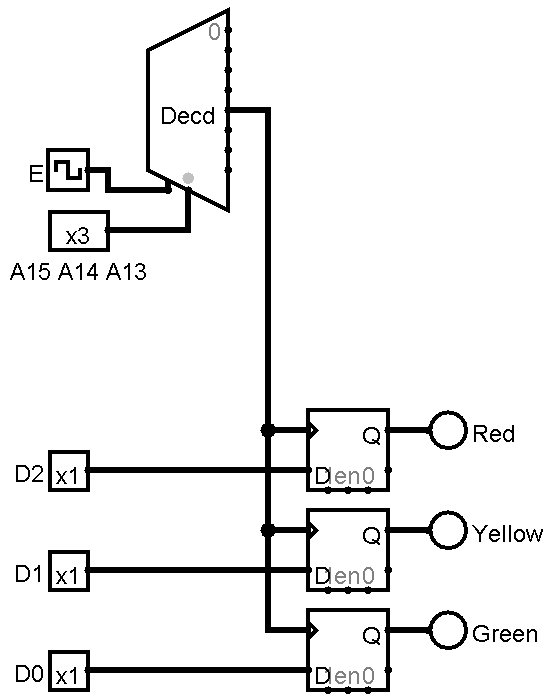
\includegraphics[scale=0.5]{hw8}
	\item [Question 2]\hspace{0pt}\\
\begin{verbatim}
Red on:
ADDA     #1
STAA     8000

Red off:
SUBA     #1
STAA     8000

Yellow on:
ADDA     #2
STAA     8000

Yellow off:
SUBA     #2
STAA     8000

Green on:
ADDA     #4
STAA     8000

Green off:
SUBA     #4
STAA     8000
\end{verbatim}
	\item [Question 3]\hspace{0pt}\\
\begin{verbatim}
      ORG      0000
loop: LDAA     #4
      STAA     8000
      JMP      C027
      JMP      C027
      JMP      C027

      LDAA     #2
      STAA     8000
      JMP      C027

      LDAA     #1
      STAA     8000
      JMP      C027
      JMP      C027
      JMP      C027
      JMP      loop
\end{verbatim}
	
	\item [\textbf{Problem 2}]\hspace{0pt}\\
	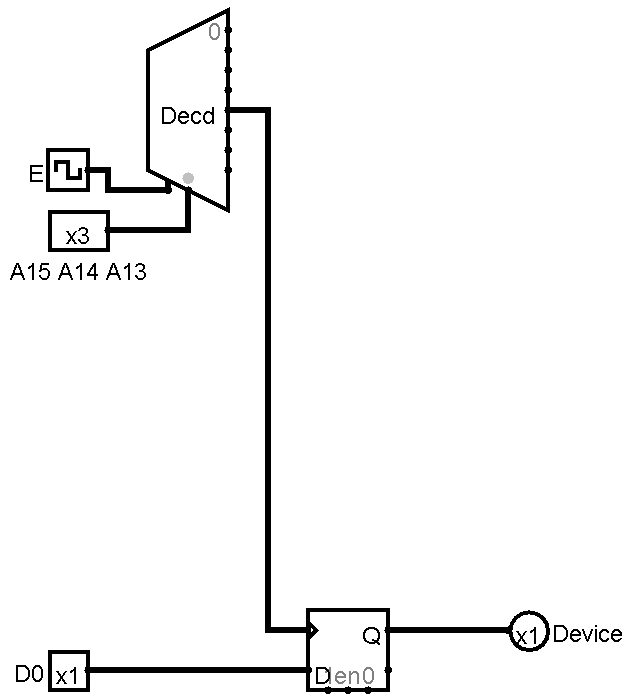
\includegraphics[scale=0.5]{hw8b}
\begin{verbatim}
      ORG      0000  ;program starts at memory address 0000
      LDAA     #0    ;initialize ACCA to 0000
loop: STAA     8000 ;send the current value of ACCA to the data bus
      INCA           ;increment ACCA
      CMPA     #64   ;check if ACCA holds 0064 (100 decimal)
      BNE      loop  ;if ACCA does not hold 0064 continue the loop
\end{verbatim}

This program will increment ACCA 100 times starting at the value 0000. This causes the first bit of the value to flip between 0 and 1 every time ACCA is incremented, resulting in 0-1-0-1-0-...1-0-1 being sent to D0 for a total of 100 alternating bits.

\end{itemize}


\end{document}